\documentclass[tikz, footheight=2em]{beamer}
\usetheme[hideothersubsections]{Hannover}
\usepackage[T1]{fontenc}
\usepackage[utf8]{inputenc}
\usepackage{amssymb}
\usepackage{amsthm}
\usepackage{amsmath}
\usepackage{color,graphicx}
\usepackage{ulem}
\usepackage{gensymb}
\usepackage{tikz}
\usepackage{algorithm}
\usepackage{algpseudocode}
\usepackage{float}
\usepackage{subfig}

\DeclareMathOperator{\card}{card}
\DeclareMathOperator{\argmax}{argmax}
\DeclareMathOperator{\uniform}{Uniform}

\usecolortheme{dolphin}

\title{QAI Tetris}
\author{C.~Cousin, G.~Hondet, L.~Pineau, B.~Viry}
\date{}

\usetikzlibrary{patterns,arrows,positioning}
\tikzset{
    %Define standard arrow tip
    >=stealth',
    %Define style for boxes
    punkt/.style={
           rectangle,
           rounded corners,
           draw=black, very thick,
           text width=6.5em,
           minimum height=2em,
           text centered},
    % Define arrow style
    pildwn/.style={
           <-,
           thick,
           shorten <=2pt,
           shorten >=2pt,},
    pilup/.style={
           ->,
           thick,
           shorten <=2pt,
           shorten >=2pt,}
}

% ----------------------------------------------------------
% nuremotation des pages -----------------------------------
% ----------------------------------------------------------
\def\swidth{1.6cm}
\setbeamersize{sidebar width left=\swidth}
\setbeamertemplate{sidebar left}
{%
  {\usebeamerfont{title in sidebar}
    \vskip1.5em
    \usebeamercolor[fg]{title in sidebar}
    \insertshorttitle[width=\swidth,center,respectlinebreaks]\par
    \vskip1.25em
  }
  {
    \usebeamercolor[fg]{author in sidebar}
    \usebeamerfont{author in sidebar}
    \insertshortauthor[width=\swidth,center,respectlinebreaks]\par
    \vskip1.25em
  }
  \hbox to2cm{\hss\insertlogo\hss}
  \vskip1.25em
  \insertverticalnavigation{\swidth}
  \vfill
  \hbox to2cm{\hskip0.6cm\usebeamerfont{subsection in
      sidebar}\strut\usebeamercolor[fg]{subsection in
      sidebar}\insertframenumber /\inserttotalframenumber\hfill}
  \vskip3pt
}
% ----------------------------------------------------------


\begin{document}

\frame{\titlepage}

\AtBeginSection[]
{%
  \begin{frame}
    \frametitle{Plan}
    \tableofcontents[currentsection]
  \end{frame}
}

\section{Apprentissage}
\subsection{Version}
\begin{frame}{Apprentissage par renforcement}
  \begin{block}{Principe}
    Un agent évoluant dans son environnement se voit attribuer des
    récompenses en fonction de la pertinence de ses actions.
    \begin{figure}[h]
      \begin{center}
        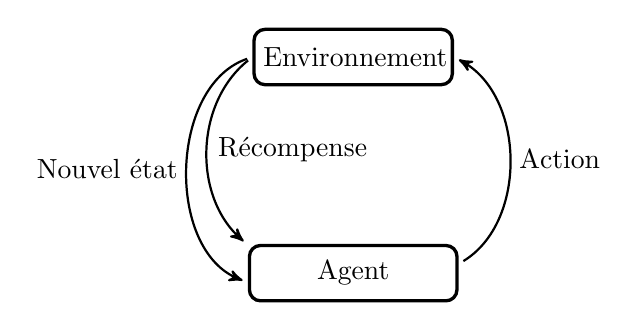
\begin{tikzpicture}[node distance=1cm, auto,]
         %nodes
          \node[punkt] (env) {Environnement};
          \node[punkt, inner sep=5pt,below=2cm of env]
          (agent) {Agent}
          edge[pilup,bend right=60] node[right] {Action} (env.east)
          edge[pildwn,bend left=70] node[left] {Nouvel état} (env.west)
          edge[pildwn,bend left=50] node[right] {Récompense} (env.west);
        \end{tikzpicture}
      \end{center}
      \caption{Principe d'apprentissage par renforcement}
      \label{fig:reinforcement_learning}
    \end{figure}
  \end{block}
\end{frame}


\subsection{Méthode employée}

\begin{frame}{Q learning}
  \begin{block}{Agent}
    Utilise une matrice Q pour stocker les espérances de récompense.
  \end{block}
  \begin{itemize}
    \item Les colonnes de la matrice correspondent aux actions.
    \item Les lignes de la matrice correspondent aux états.
  \end{itemize}
\end{frame}

\subsection{Choix de l'action}

\begin{frame}{État}
  Données utiles de l'environnement pour jouer une action.

  \begin{block}{Obtention}
    \[
      \text{plateau} \pause{} + \text{pièce} \pause{} = \text{état}
      \pause{} \in \mathbf{N}
    \]
  \end{block}
\end{frame}

\begin{frame}{Choix de l'action}
    \(Q(s, a)\) approxime la récompense a long terme,
    \pause{}
    \[ \text{action choisie} = \argmax_a Q(s, a) \]
    \pause{}
  \begin{algorithm}[H]
      \caption{Choix de l'action}\label{alg:action}
      \begin{algorithmic}
        [1]
        \Procedure{ChooseAction}{$Q$, $s$, $\mathcal{A}$}
        \State{} tirage \(\gets \uniform([0, 1])\)
        \If{tirage \(> \epsilon\)}
        \Return{\(\argmax_{a\in\mathcal{A}} Q(s, a)\)}
        \Else{}
        \Return{\(\uniform(\mathcal{A})\)}
        \EndIf{}
        \EndProcedure{}
      \end{algorithmic}
  \end{algorithm}
\end{frame}

\section{Environnement Tetris}
\subsection{Tetromino}
\begin{frame}[c]{Tetromino}
  \begin{block}{Représentation}
    Matrice \(2 \times 2\) d'entiers
  \end{block}
  \begin{figure}[h]
    \centering
    \subfloat[Diagonale] {%
      
\begin{tikzpicture}
        \fill[color=magenta] (0,0) rectangle (1,1);
        \fill[color=magenta] (0,0) rectangle (-1,-1);
        \draw (-1,1) rectangle (1,-1);
      \end{tikzpicture}
    }\qquad
    \subfloat[L] {%
      
\begin{tikzpicture}
        \fill[color=cyan] (0,0) rectangle (1,1);
        \fill[color=cyan] (0,0) rectangle (-1,-1);
        \fill[color=cyan] (0,0) rectangle (-1,1);
        \draw (-1,1) rectangle (1,-1);
      \end{tikzpicture}
    }\qquad
    \subfloat[Carré] {%
      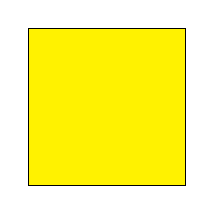
\begin{tikzpicture}
        \fill[color=yellow] (0,0) rectangle (1,1);
        \fill[color=yellow] (0,0) rectangle (-1,-1);
        \fill[color=yellow] (0,0) rectangle (-1,1);
        \fill[color=yellow] (0,0) rectangle (1,-1);
        \draw (-1,1) rectangle (1,-1);
      \end{tikzpicture}
    }\\
    \subfloat[Barre] {%
      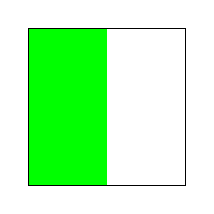
\begin{tikzpicture}
        \fill[color=green] (0,0) rectangle (-1,-1);
        \fill[color=green] (0,0) rectangle (-1,1);
        \draw (-1,1) rectangle (1,-1);
      \end{tikzpicture}
    }\qquad
    \subfloat[Point] {%
      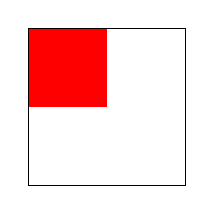
\begin{tikzpicture}
        \fill[color=red] (0,0) rectangle (-1,1);
        \draw (-1,1) rectangle (1,-1);
      \end{tikzpicture}
    }
    \caption{Liste des tetrominos}\label{fig:tetrolist}
  \end{figure}
\end{frame}

\subsection{Action}
\begin{frame}[c]{Action}
  \begin{block}{Définition}
    Données utiles au placement d'un tetromino sur le plateau.
    \[ \text{action} = \text{orientation} + \text{translation} \]
  \end{block}

  \begin{block}{Types}
    \begin{itemize}
      \item translation \(\in [0, 5]\)
      \item orientation \(\in \{\)North, South, East, West\(\}\)
    \end{itemize}
  \end{block}
  \begin{alertblock}{Tetromino flottant}
    schema here. Un ensemble d'orientations par tetromino.
  \end{alertblock}
\end{frame}

\subsection{Gestion du plateau}
\begin{frame}[c]{Réalisation de l'action et conséquences}
  \begin{block}{Placement vertical}
    Évaluation des collisions: collision \(\rightarrow\) placé en amont
  \end{block}
  \begin{block}{Lignes pleines}
    Ligne remplie enlevée du jeu
  \end{block}
\end{frame}

\section{Évolution de l'agent}
\subsection{Récompense}
\subsection{Mise a jour}
\subsection{Resultats}
\subsection{Paametrage}


\section{Valuation}

\end{document}
